\chapter{Design and Implementation}
\label{design}
In this chapter we introduce a novel model for Compositional Data Analysis. It combines dimensionality reduction and supervised learning into a single, end-to-end algorithm. This design is motivated by the drawbacks of traditional methods, such as PCR. Such methods obtain the low level representation independently of the training targets, and so may ignore information which can improve the predictive performance. We divide this chapter into the following sections: 

\begin{itemize}
    \item Section \ref{design}: Here we present a high level overview of the model, including the assmuptions, inputs and outputs. 
    \item Section  \ref{endloss}: This section describes in detail the loss function(s) which the model is optimising.
    \item Section \ref{architecture}: The full architecture of the model is outlined here. We also detail the computations involved in a forward pass of the model. 
    \item Section \ref{implementation}: The implementation details of the model are presented and discussed here. We also detail the Python package for this code, which is available online.
\end{itemize}
\pagebreak



\section{Model Overview}
\label{design}
The application of our model is to supervised learning problems where the features form a compositional data set. The targets are currently restricted to single real valued numbers (regression), or classification problems (either single or multi class). Formally, the model takes as input a compositional matrix $\mathbf{X} \in \mathbb{R}^{n \times d}$ with each $x_i \in S^{d-1}$.  The output of the model is a prediction $\hat{\mathbf{y}}$ of the true targets $\mathbf{y}$. In the regression case, the targets are $\mathbf{y} \in \mathbb{R}$, and for classification $\mathbf{y} \in \{0, ..., k\}$ where $k$ is the number of classes. The prediction is generated from the following two steps:
\begin{itemize}
    \item Reduce $X$ to a representation $A \in \mathbb{R}^{n \times l}$ where $l < d$, through the mapping $\Theta(X) = A$.
    \item Use $A$ as input to the prediction mapping, which we denote as $r(A) = \mathbf{\hat{y}}$.
\end{itemize}

\todo{Introduce notation. How you stack elements into vectors, vectors into matrices, bold, non-bold, etc}

We can then define the end-to-end mapping from $X$ to $\mathbf{\hat{y}}$ as the composition of the above functions:
\begin{align}
\label{forwardpass}
    f(X) = r(\Theta(X)) = r(A) = \mathbf{\hat{y}}
\end{align}

\section{End to End Loss}
\label{endloss}
The steps outlined above for the forward pass are common to many supervised learning approaches, such as PCR which also performs regression on a low level representation. The novelty of our approach is the loss function under which $f(X)$ is optimised. In typical applications, the encoding $\Theta(X)$ and the prediction $r(A)$ are separately optimised with respect to different criteria. To account for this, our model instead directly optimises the composition $f(X)$ under a single loss function. \\
\fix{Careful of bold vs non-bold. E.g. $x_i$, $\mathbf{\hat{y}}$, $\hat{y}$}
To define this loss function we first recall the regression and classification loss from \ref{sec:sup}, and the CoDA-PCA loss from \ref{codapca}. For predictions $\hat{y}$, targets $y$, reconstruction $Y$ and geometrically normalised data $\check{X}$ we have: 
\begin{align}
    l_{regression} &= ||\hat{y} - y ||^2_2 \\
    l_{classification} &= %NLL loss
    \\
    l_{CoDA-PCA} &=   \mathbf{1}^T\exp{(\mathbf{Y})}\mathbf{1} + \text{tr}(\check{\mathbf{X}}^T\mathbf{Y})
\end{align}
\fix{3.3 definition}
\fix{Suggest $l_{\mathrm{regression}}$ instead of $l_{regression}$}
We have mentioned that our model is an end to end solution for dimensionality reduction and supervised learning. This is done is by combining the reconstruction loss $l_{CoDA-PCA}$ with a supervised loss, $l_{regression}$ or $l_{classification}$. This combination is taken as a weighted sum of the reconstruction and supervised losses, with a scaling parameter $\lambda$. We note that all the above loss functions are differentiable, and so the weighted sum is differentiable.

Formally, given a reconstruction loss $l_{x}$, supervised loss $l_{y}$, and a scalar $\lambda \in \mathbb{R}$ we define the end-to-end loss as:  
\begin{align}
    l_{end-to-end} = l_{y} + \lambda l_{x}
\end{align}

We note that this concept can be applied to any choice of reconstruction or supervised loss $l_{x}$ or $l_{y}$, however we focus on the CoDA case with single valued regression and mulit-class classification. We can now proceed to define the specific loss functions for each case.   


\subsection{CoDA-Regress}

In the regression case, we are given targets and predictions $y, \hat{y} \in \mathbb{R}$. We can then define the algorithm $CoDA-Regress$, with the corresponding loss function defined as:  
\begin{align}
   l_{CoDA-Regress} =||\hat{y} - y||^2_2 + \lambda  \left(\sum_{i=1}^n\sum_{j=1}^m\exp{Y_{ij}} + \text{tr}(\check{X}^TY)\right) 
\end{align}

\subsection{CoDA-Cl}

Similarly, for a classification problem with targets and predictions $\hat{y}, y \in \{1,...,k\}$, we define the loss function for the algorithm $CoDA-Cl$:  
\begin{align}
   l_{CoDA-Regress} = NLL + \lambda  \left(\sum_{i=1}^n\sum_{j=1}^m\exp{Y_{ij}} + \text{tr}(\check{X}^TY)\right) 
\end{align}

\section{Model Architecture}
\label{architecture}
We are now in a position to fully describe the architecture of the model. Recall the forward pass from \ref{forwardpass}: 

\begin{align*}
    f(X) = r(\Theta(X)) = r(A) = \mathbf{\hat{y}}
\end{align*}

Both $\Theta$ and $r$ are implemented as fully connected networks, to which we associate the weights $\mathbf{w}_\Theta$  and $\mathbf{w}_r$. We additionally define a decoder network $U$ with weights $\mathbf{w}_U$. This network takes as input the representation $\Theta(X) = A$, and outputs a reconstruction $Y$ of $X$ in the original domain. This autoencoder structure was inspired by the CoDA-AE algorithm in \cite{Avalos2018}. Although not necessary for the forward pass, the reconstruction is needed for optimisation of the model weights. These model weights are  given by the union of the above networks: 

\begin{align}
    \mathbf{W}_f = \{\mathbf{w}_\Theta\} \cup \{\mathbf{w}_r\} \cup \{\mathbf{w}_U\}
\end{align}

These weights are optimised with respect to the end-to-end loss functions defined in \ref{endloss}. Given these functions are differentiable, they can be optimised by any gradient based optimisation algorithm. Algorithm \ref{Alg1} details the high level training cycle of the model. Figure \ref{fig:model} outlines the information flow for computing the combined loss. \\\\


\begin{algorithm}[H]
\SetAlgoLined
\SetKwInput{Kw}{input}
\Kw{Compositional data matrix $X$, initialisation matrix $I$, ground truth $y$, scalar $\lambda$, optimiser $O$, epochs $n$}
\SetKwInput{Kw}{output}
\Kw{Trained model weights $\mathbf{W}_f$}

\SetKwInput{Kw}{input}
$\mathbf{W}_f = \mathbf{I}$  \;
 $epoch = 0$ \;
 \While{$epoch < n$}{
    $A = \Theta(X)$\;
    $\hat{y} = g(A)$ \;
    $Y = U(A)$\;
    $l_{CoDA-PCA} = \mathbf{1}^T\exp{(Y)}\mathbf{1} + \text{tr}(\check{X}^TY)$ \;
    $l_x = l_{CoDA-PCA}$\;
  \eIf{$y \in \mathbb{R}$}{
    $l_y = ||\hat{y} - y||^2_2$\;

  }{    $l_y = NLL$\;
  }
  $l_{coda-to-end} = l_y + \lambda l_x$ \;
  $\mathbf{W}_f = O(\mathbf{W}_f, l_{coda-to-end}) $ \;
  $epoch = epoch + 1$ \;
 }
 \caption{coda-to-end: An end-to-end model for CoDA}
 \label{Alg1}
\end{algorithm} ~\\\\

If we only optimise this network with respect to the supervised loss $l_y$, it leads to representations $A$ which do not faithfully represent the data. We see this result experimentally in \ref{}. This can then lead to a decrease in the performance of the regression, since the representation is not accurate. This motivates the addition of the reconstruction loss $l_x$, which in many ways is similar to a regularisation term. By ensuring the encoding will not deviate too far from the ideal representation, the model performance can be improved.   



\begin{figure}
    \centering
    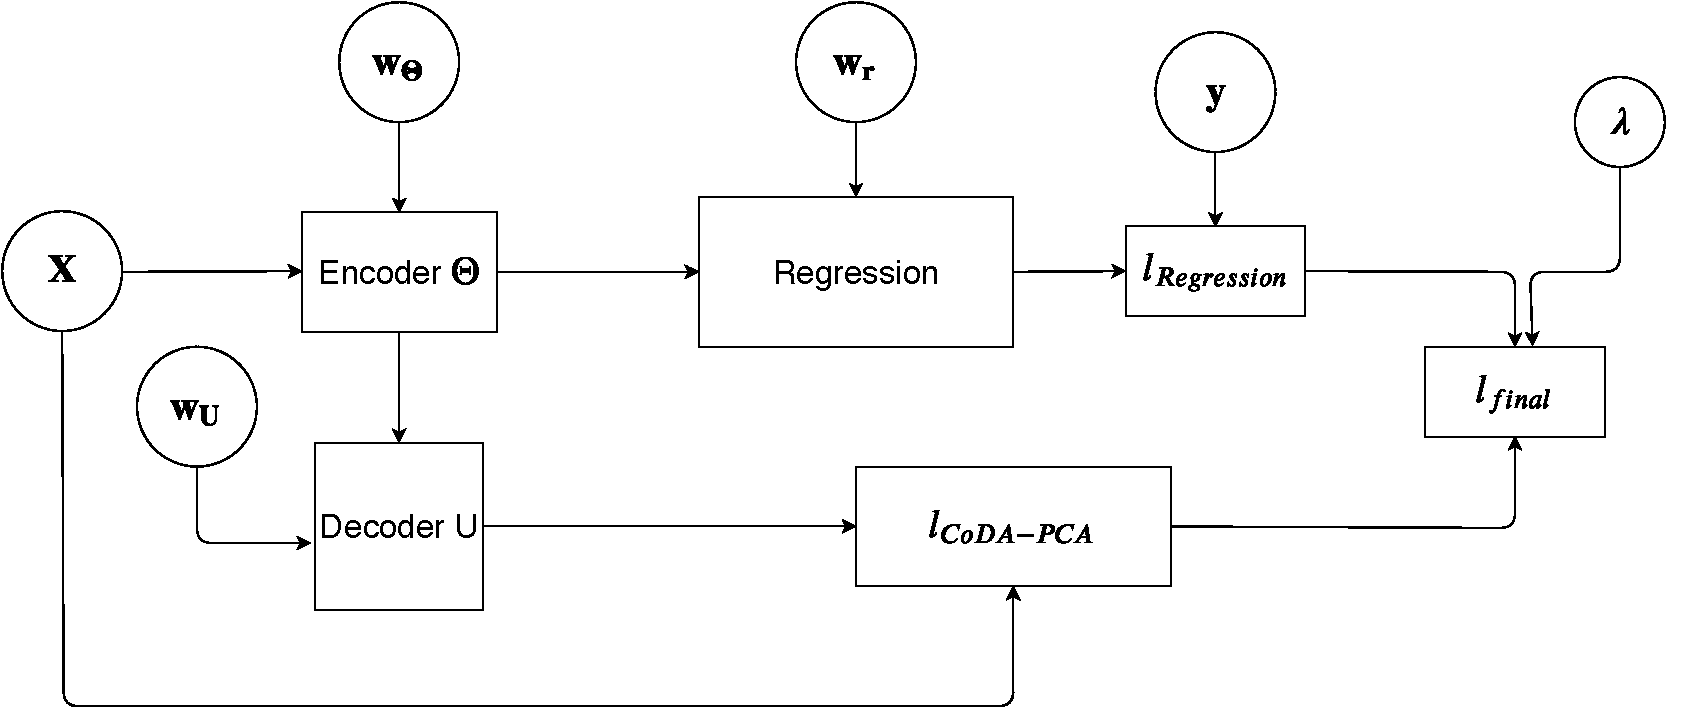
\includegraphics[width=17cm]{figs/codadiagram.pdf}
    \caption{End to End ("Coda-to-end") Model Diagram}
    \label{fig:model}
\end{figure}

% Description of symbols:\\
% $\bf X$: Input Matrix\\
% $\bf{w_\Theta}$: Parameters for Encoding Network \\
% $\bf{w_U}$: Parameters for Decoding Network\\
% $\bf{w_r}$: Parameters for Regression\\
% $\bf{y}$: Target vector\\
% $\lambda$: Regularisation parameter, controlling how much to weight reconstruction error
% \\\\





\section{Implementation}
\label{implementation}
The model defined in \ref{architecture} was implemented in PyTorch, with the source code available on GitHub. A high level outline of the implementation is as follows: The algorithms CoDA-Regress and CoDA-Cl form the basis for the code, and are each implemented as a separate class. The user defines the desired low level dimension, as well as the encoder and decoder dimensions. Using these parameters, an ordered dictionary is used to stack the layers for the encoder and decoder to ensure the correct ordering of dimensions. This includes the nonlinearities, for which we use Exponential Linear Units (ELUs). These dictionaries are then used as input to the  PyTorch Sequential module to format them as PyTorch objects. \\

The output layer is algorithm specific. CoDA-Regress has a linear layer mapping to a single output, which is the predicted regression value. CoDA-Cl has a linear layer mapping to the number of classes followed by a log softmax layer, which gives the log probabilities for each class. \\

The forward pass is as described in \ref{architecture}, with the input being modified to contain both the original matrix $X$ and $X_{ckl} = \log \check{X}$. This is done as per \cite{Avalos2018}. \\

The optimisation is done using Adam \citep{}. Referring to algorithm \ref{Alg1}, this takes the place of the function $O$. We found this to be more numerically stable during experiments in comparison to standard Stochastic Gradient Descent (SGD), in addition to faster convergence. 

\subsection{CoDA-PCA Package}

We see from \citep{Avalos2018}, CoDA-PCA gives a significant improvement in dimensionality reduction over current methods. Although the code for this paper is available, it has not yet been packaged to production standards. We have reimplemented and packaged the code from \citep{Avalos2018}, along with the CoDA-Regress and CoDA-CL algorithms presented here. These are available on the Python Packaging Index (PyPI), with easy installation using pip. These algorithms can be accessed using a simple API, which allows users to benefit from their advantages over related algorithms.   \todo{add documentation etc. of package?}



\section{Summary}
We have introduced the algorithms CoDA-Regress and CoDA-Cl for supervised learning problems with compositional features. 
Given a feature vector $\bf X$ and target vector $\bf y$, these models fit predictions using a low dimensional representation of the original data. The final loss is computed as the sum of the supervised loss $l_{y}$ and the reconstruction loss $l_{x}$, with the reconstruction loss being scaled by a real valued parameter $\lambda$.  



